%! TEX root = analisis_kaitan_temu7.tex
% the main TeX file which is intended to compile, :VimtexReload after adjustment
% :h vimtex-tex-root
\documentclass[../main.tex]{subfiles}
% \includeonlyframes{current}
% \setbeameroption{hide notes} % Only slides
% \setbeameroption{show only notes} % Only notes
% \setbeameroption{show notes on second screen=right} % Both

\begin{document}

\bgdarkimg{kaitan_1}
\begin{frame}[mytitle=standard,c,mycolor=digiPH_ubcblue,dark]
	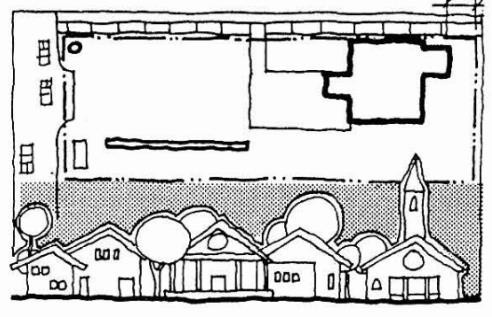
\includegraphics[width=.71\textwidth]{../figures/kaitan_2}
\end{frame}

\begin{frame}[mytitle=standard,t,mycolor=digiPH_gray,light]
	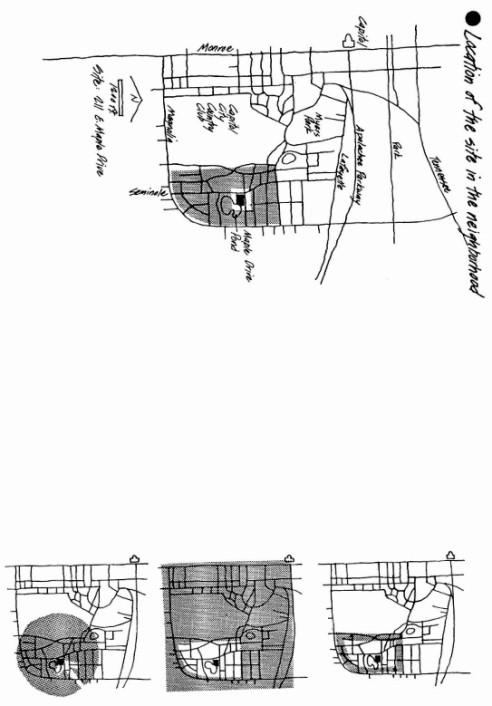
\includegraphics[width=.71\textwidth, angle=90]{../figures/kaitan_3}
\end{frame}

\begin{frame}[mytitle=standard,t,mycolor=digiPH_gray,light]
	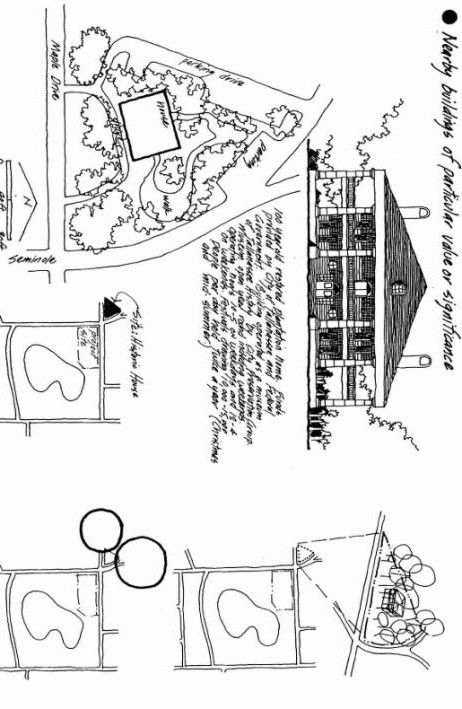
\includegraphics[width=.71\textwidth, angle=90]{../figures/kaitan_4}
\end{frame}

\begin{frame}[mytitle=standard,t,mycolor=digiPH_gray,light]
	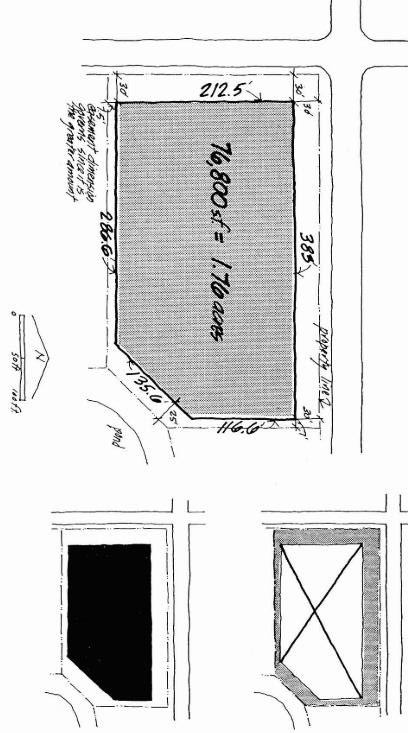
\includegraphics[width=.71\textwidth, angle=90]{../figures/kaitan_5}
\end{frame}

\begin{frame}[mytitle=standard,t,mycolor=digiPH_gray,light]
	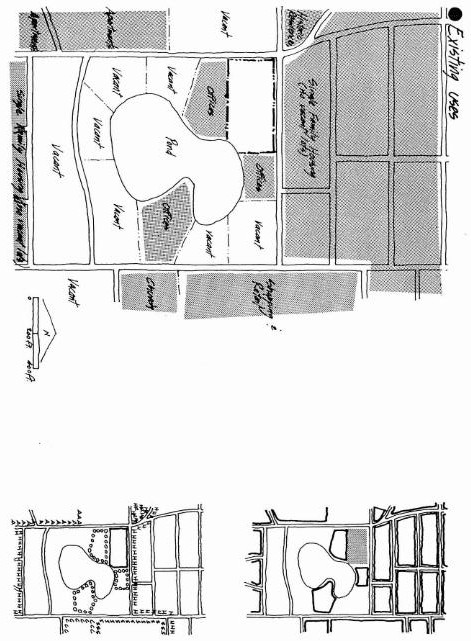
\includegraphics[width=.71\textwidth, angle=90]{../figures/kaitan_6}
\end{frame}

\begin{frame}[mytitle=standard,t,mycolor=digiPH_gray,light]
	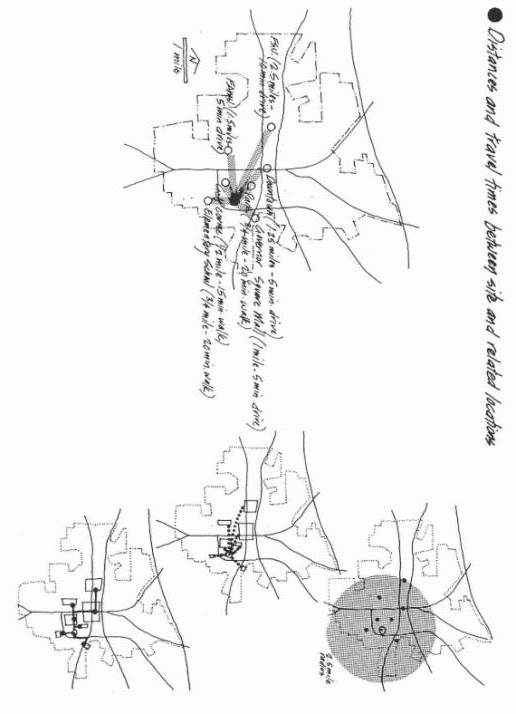
\includegraphics[width=.71\textwidth, angle=90]{../figures/kaitan_7}
\end{frame}
\bgdarkimg{kaitan_8}


\bgdarkimg{kaitan_cth}
\bgdarkimg{lingkungan_cth}
\bgdarkimg{akses_lingkungan_bising_cth}

\end{document}
